\noindent The following images show the most important screens of the application.
\bigskip
\subsection{Homepage and Search Path}
The homepage is the first screen displayed after logging in. From this screen, the user can search for a path by entering the starting point, the destination, and a tolerance level. By clicking Search Path, the results are displayed in order of score. Below the search results, there is a section showcasing the top-rated paths. When the cyclists clicks on a specific path, the Path's Details page is shown.
\begin{figure}[H]
\centering
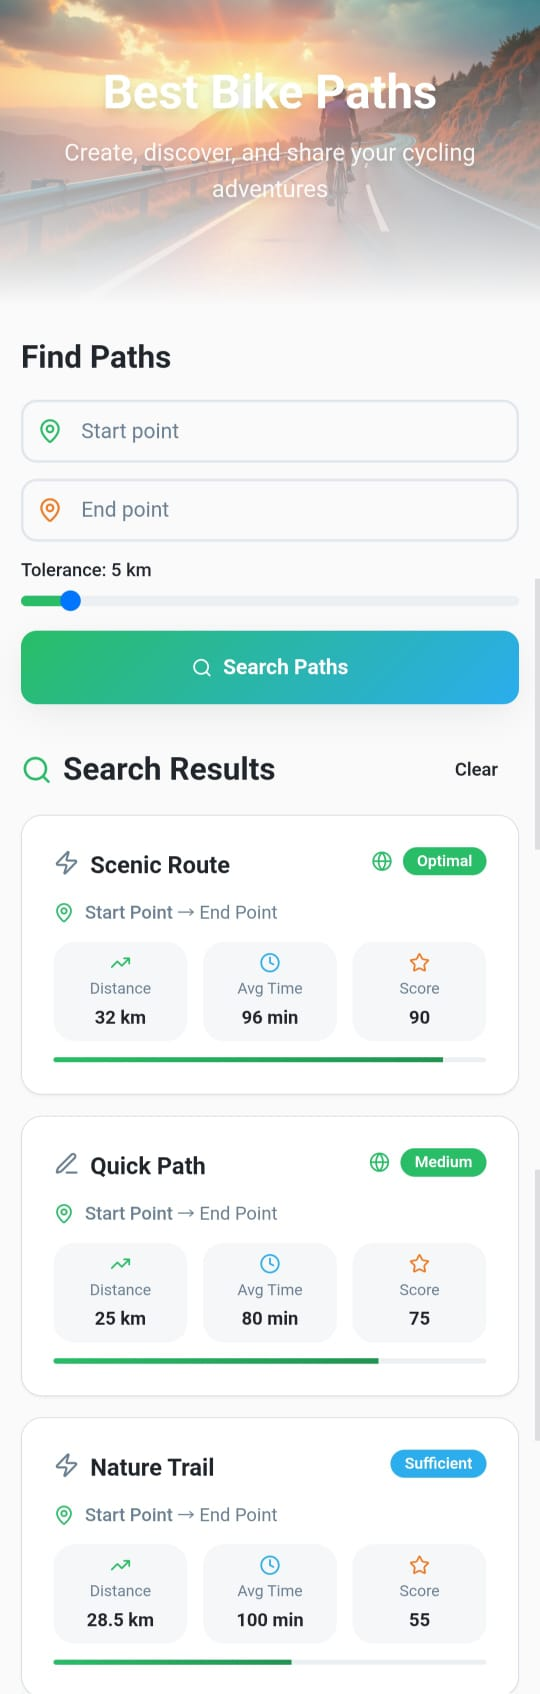
\includegraphics[width=0.35\linewidth]{Images/UserInterface/Search1.jpeg}
\hspace{1.3cm}
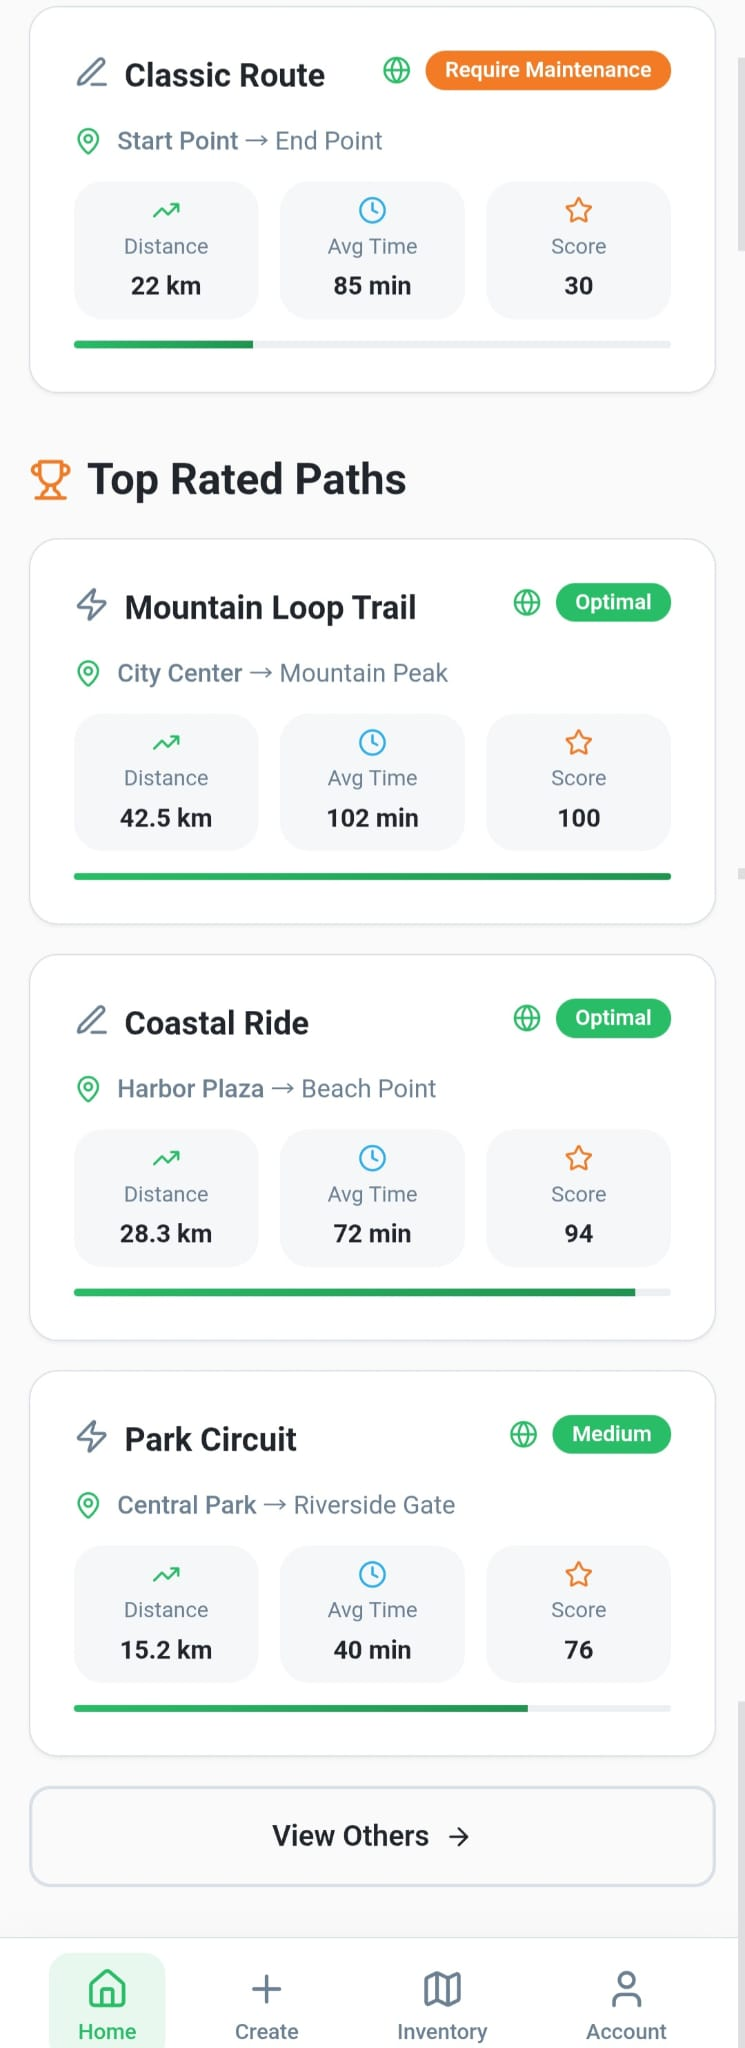
\includegraphics[width=0.35\linewidth]{Images/UserInterface/Search2.jpeg}
\caption{Screens of Homepage, \textit{Search Paths}}
\label{fig:Homepage}
\end{figure}
\newpage
\subsection{Navigation}
The navigation screen allows the user to view a map to follow a selected path. Buttons below the map let the user pause or stop the navigation. In real time, the app displays information such as time, distance, speed, and remaining distance.
\begin{figure}[H]
\centering
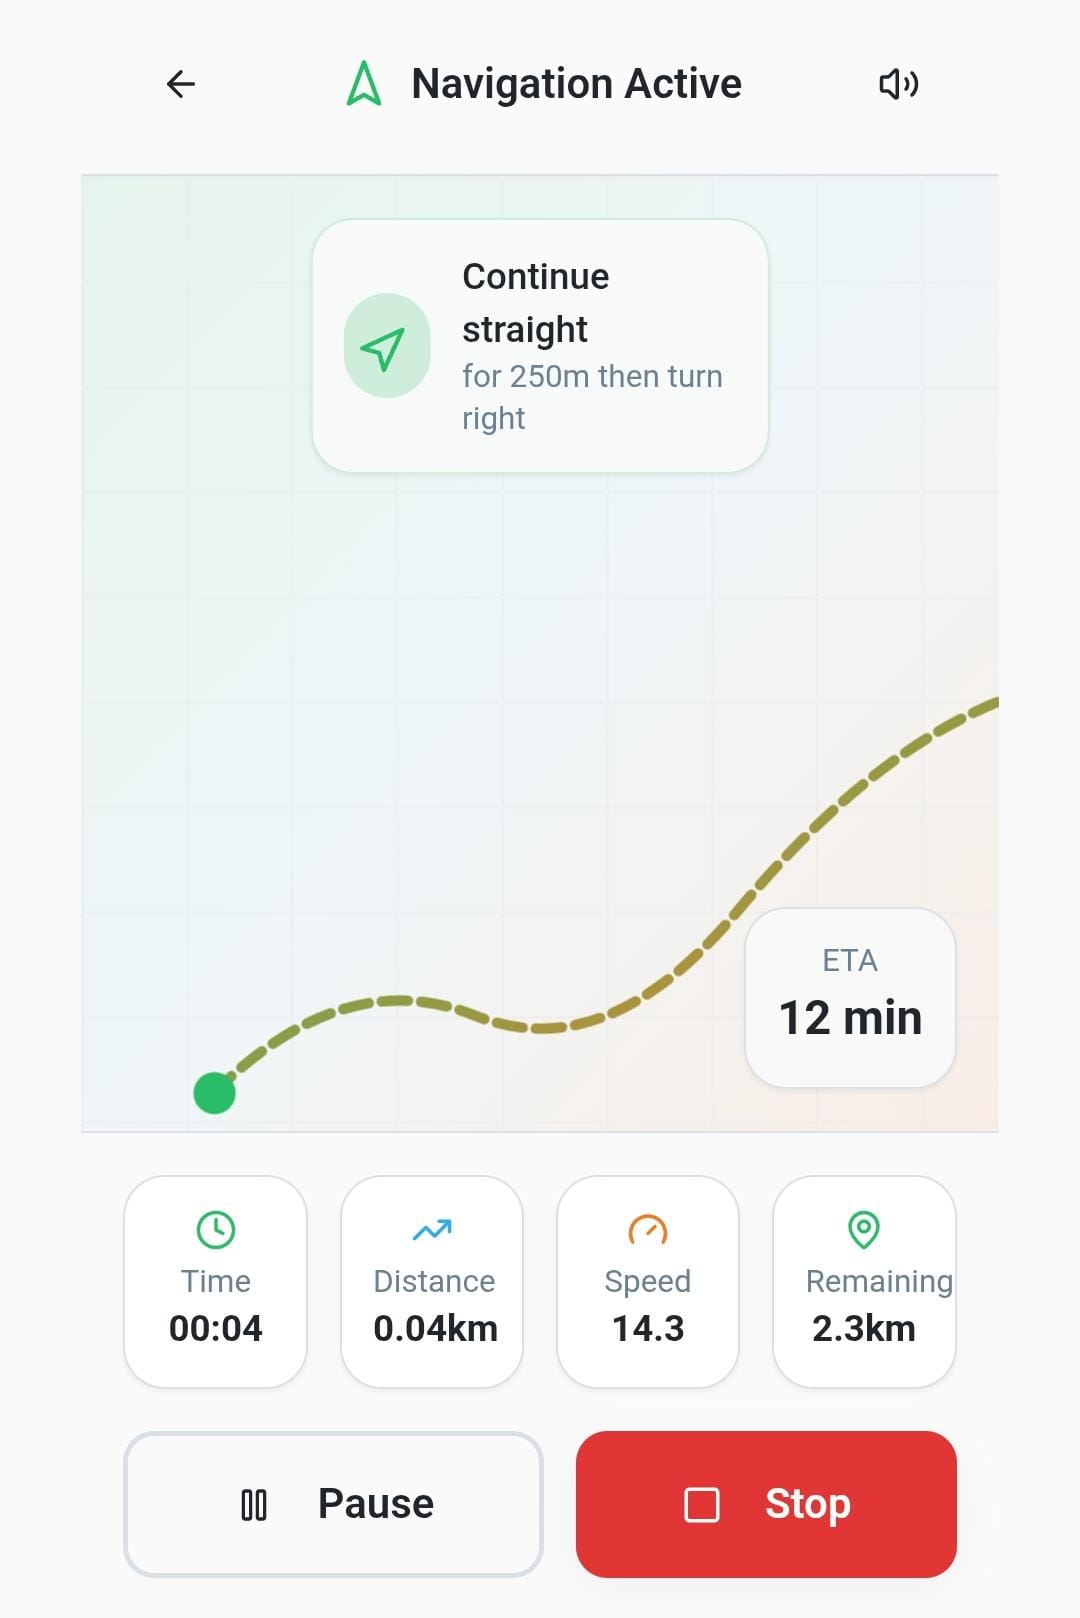
\includegraphics[width=0.35\textwidth]{Images/UserInterface/Navigation.jpeg}
\caption{Screen of \textit{Navigation}}
\label{fig:Navigation}
\end{figure}
\newpage
\subsection{Authentication: Login and Sign-Up}
The login page is used to access the BBP app when the user is registered. This page includes the following key elements:
\begin{itemize}
    \item \textbf{Email Field:} a text input field where users enter their registered email address.
    \item \textbf{Password Field:} a secure input field for users to enter their password.
    \item \textbf{Login Button:} a button that, when clicked, authenticates the provided credentials and, if correct, grants access to the platform. In this moment the application shows the Homepage.
\end{itemize}
\noindent The sign up page is used to access the BBP app when the user is not registered. This page includes the following key elements:
\begin{itemize}
    \item\textbf{Name Field:} a text input field where users enter their Name
    \item \textbf{Email Field:} a text input field where users enter their email address.
    \item \textbf{Password Field:} an secure input field for users to create their password.
    \item \textbf{SignUp Button:} a button that, when clicked, create e new a account. 
\end{itemize}
\begin{figure}[H]
\centering
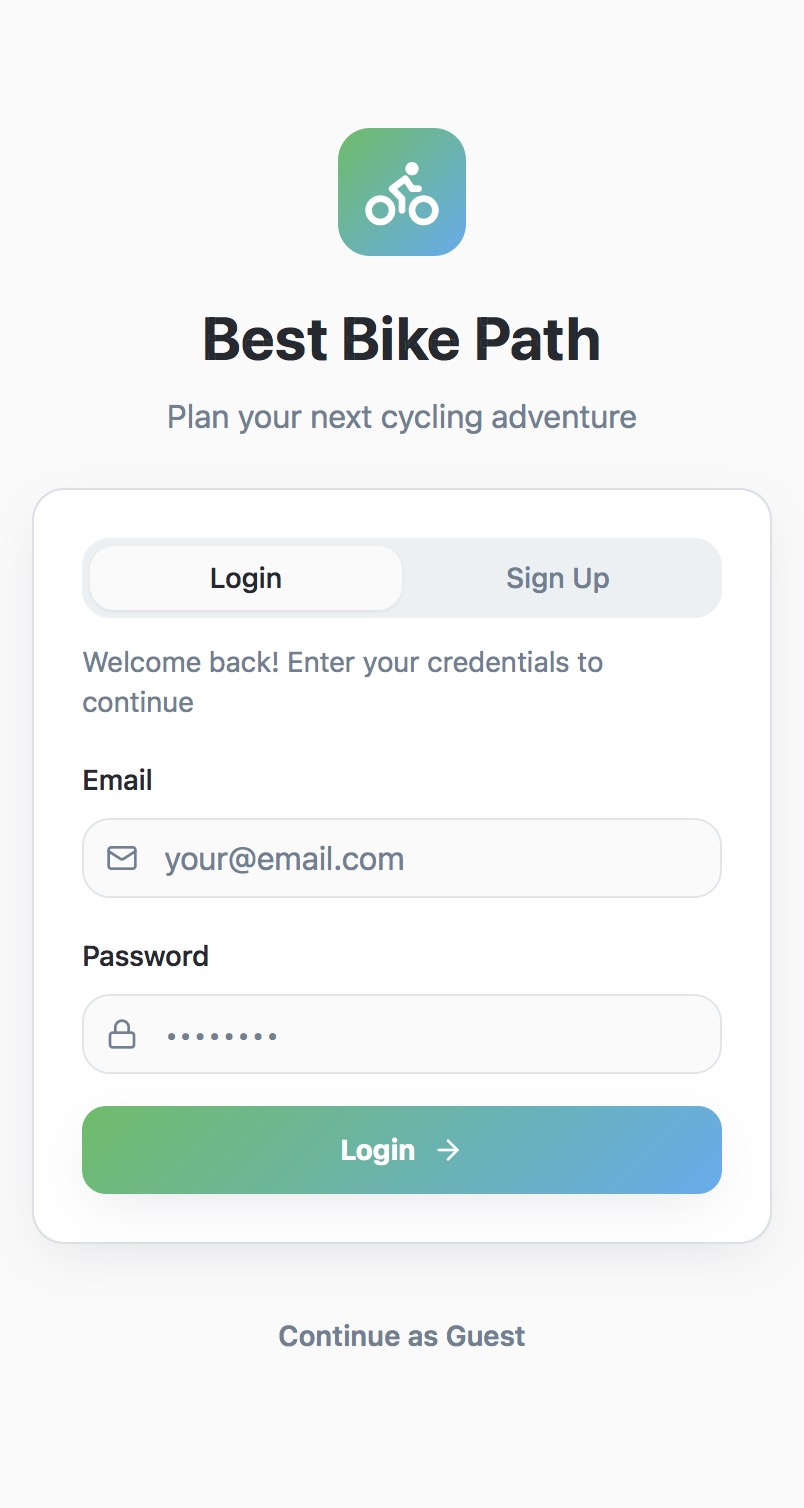
\includegraphics[width=0.35\textwidth]{Images/UserInterface/SignUp.JPG}
\hspace{1.3cm}
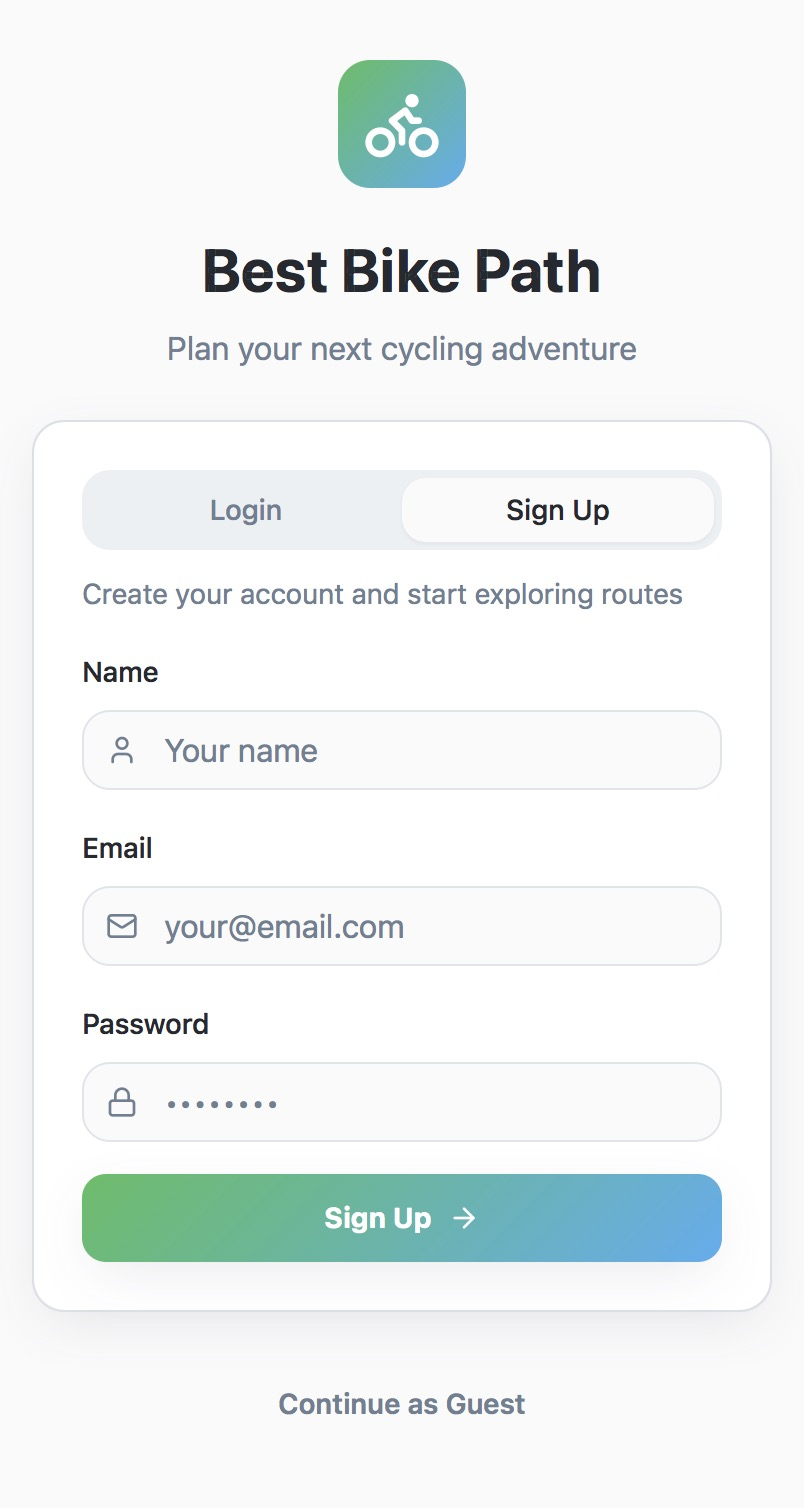
\includegraphics[width=0.35\textwidth]{Images/UserInterface/Login.JPG}
\caption{Screens of the Authentication, \textit{Login} and \textit{SignUp}}
\label{fig:LoginSignUp}
\end{figure}
\newpage
\subsection{Account and Edit Account}
By clicking the Account button located at the bottom of the screen, the cyclist can access and view their personal profile.
This screen displays all statistics related to the cyclist’s recorded paths. In addition, it includes a Delete Account button, which allows the cyclist to permanently delete their account.
The cyclist can also choose to update their personal information by selecting the Edit Account button. After pressing this button, the Edit Account page is displayed, where the cyclist can modify their name, email address and password.
\begin{figure}[H]
\centering
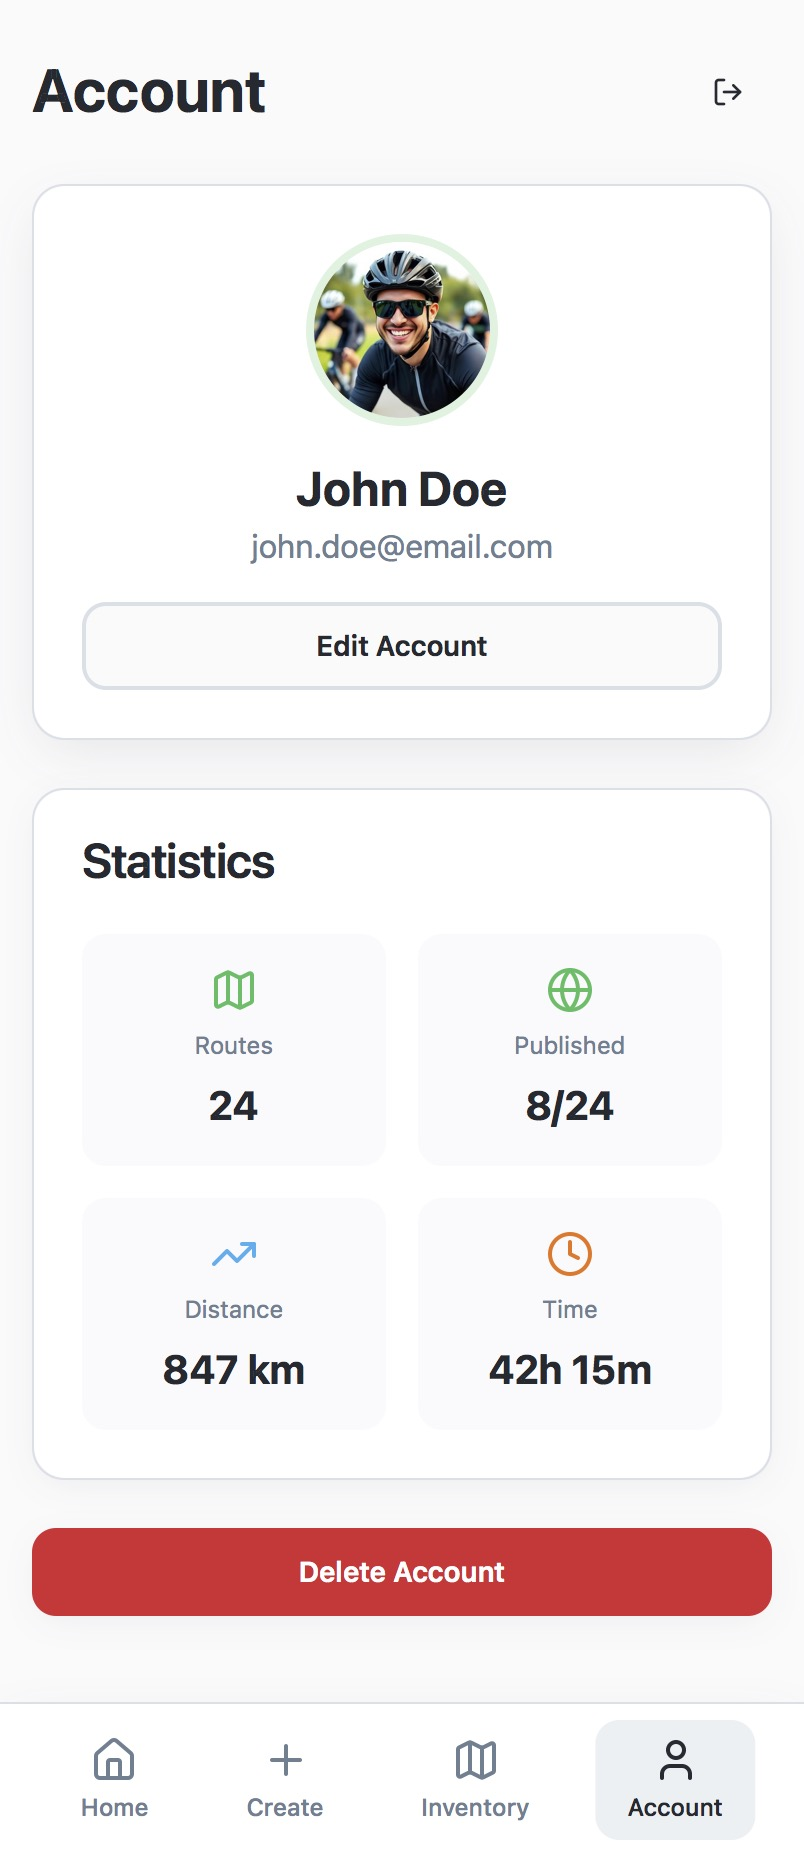
\includegraphics[width=0.4\textwidth]{Images/UserInterface/Account.JPG}
\hspace{1.3cm}
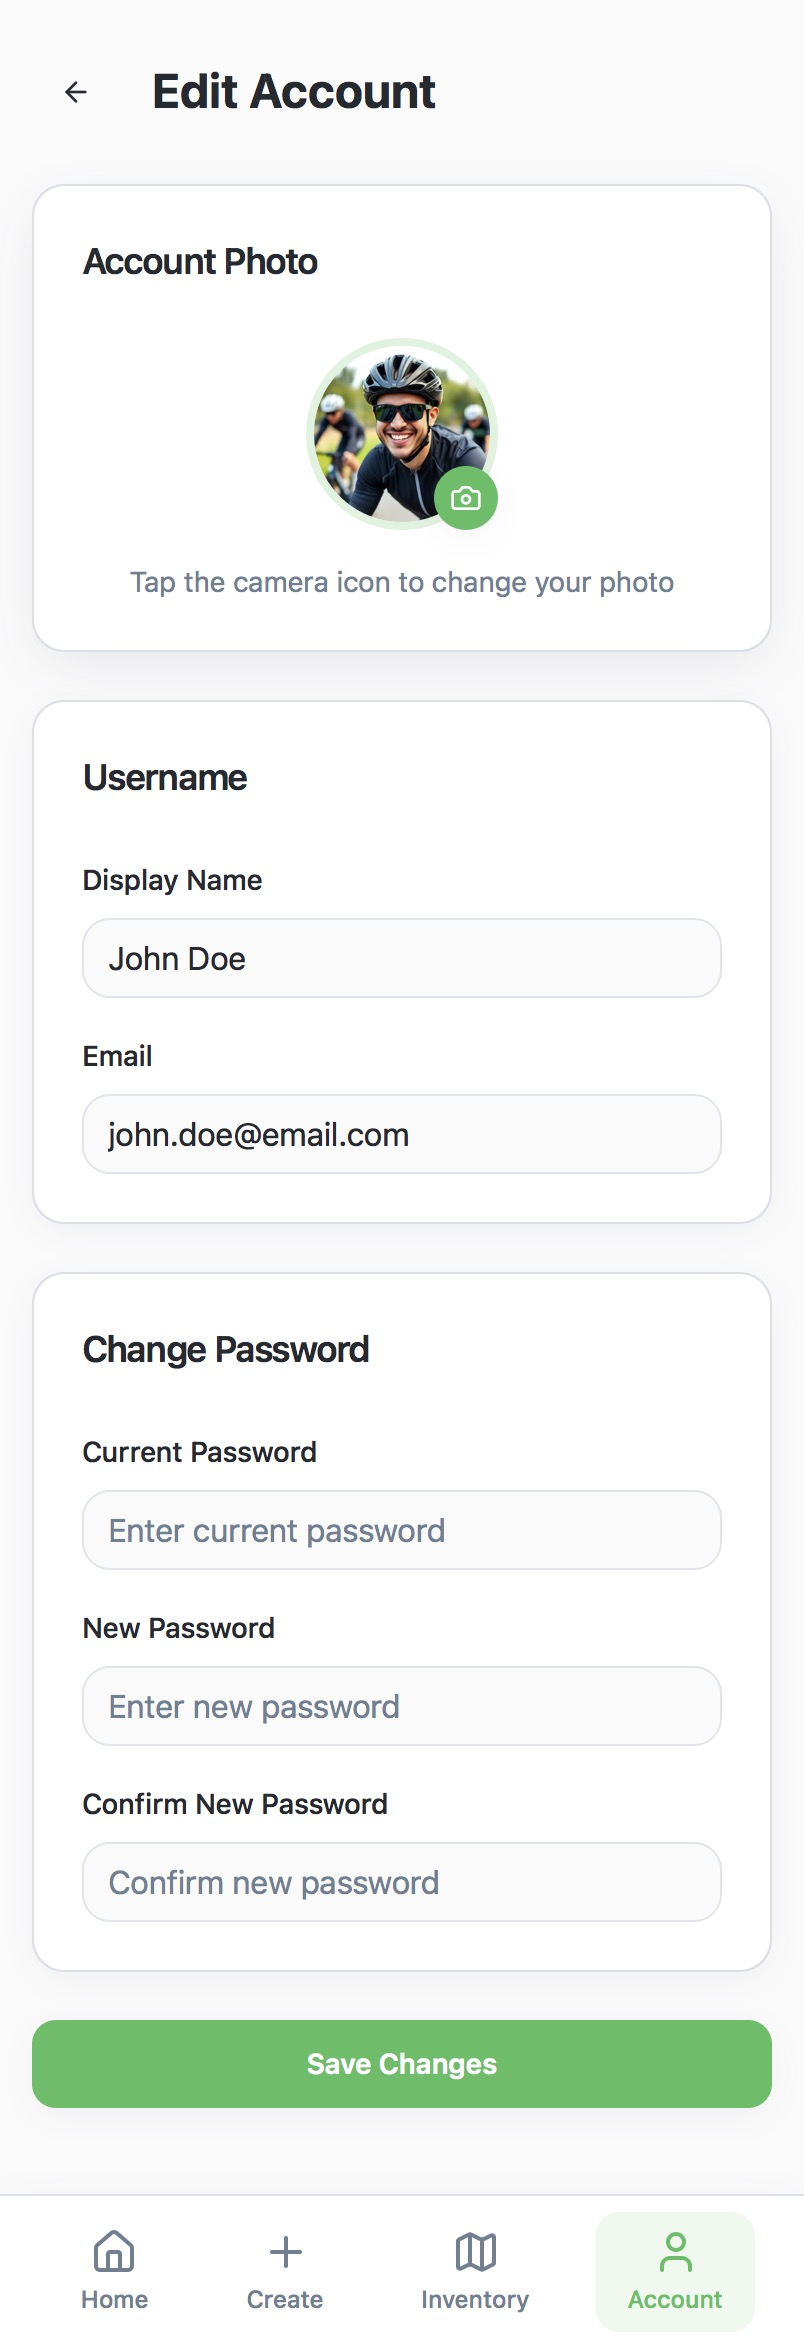
\includegraphics[width=0.4\textwidth]{Images/UserInterface/EditAccount.JPG}
\caption{Screens of \textit{Account} and \textit{Edit Account}}
\label{fig:Account}
\end{figure}
\newpage
\subsection{Inventory and Path's Details} 
The Inventory page allows cyclists to view all their previously recorded paths, along with the related statistics. By selecting a specific path, the Path Details page is displayed. This page shows all the routes associated with the selected path. From this screen, the cyclist can start a new navigation by clicking the Start Navigation button, which enables them to follow the selected path.
\begin{figure}[H]
\centering
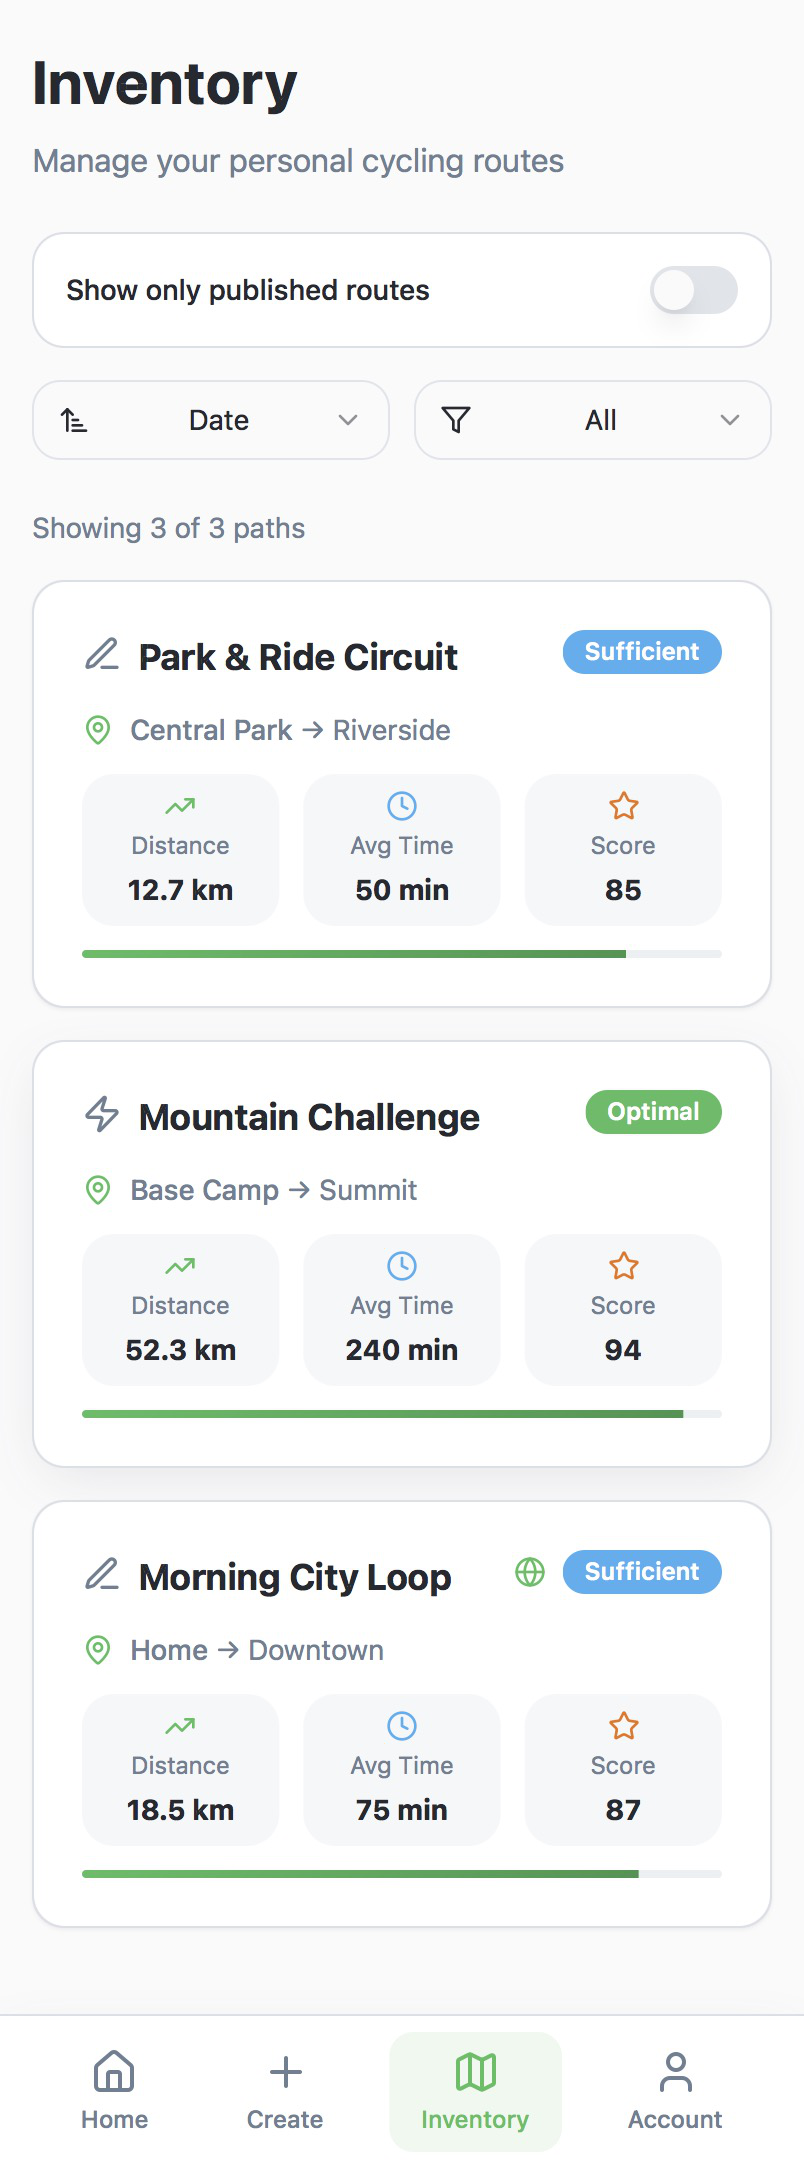
\includegraphics[width=0.4\textwidth]{Images/UserInterface/inventory.png}
\hspace{1.3cm}
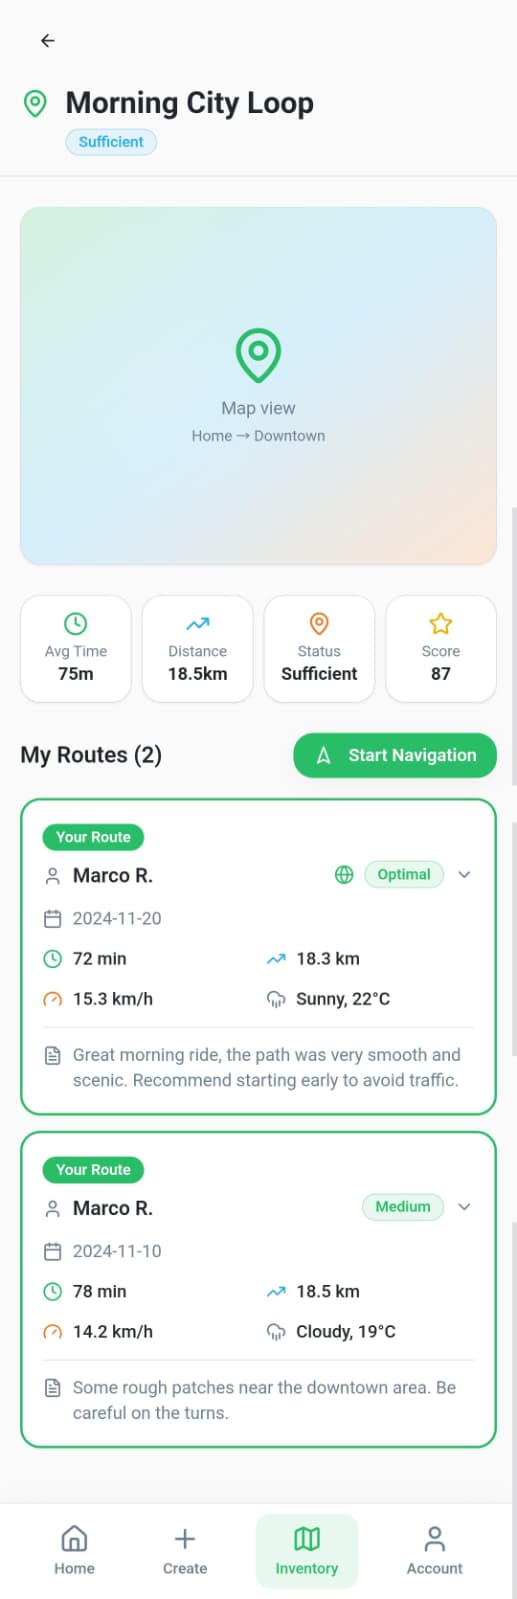
\includegraphics[width=0.4\textwidth]{Images/UserInterface/MyRoute.jpeg}
\caption{Screens of \textit{Inventory} and \textit{Path's details}}
\end{figure}
\subsection{Create route}
The Create Route page presents the cyclist with the route creation modes supported by the application. Specifically, the application offers two options: Manual Mode and Automatic Mode. \\
Based on the creation mode selected by the cyclist, the system displays either the Automatic Route Creation page or the Manual Route Creation page.\\
The Create Route (Automatic) page provides a Start Tracking button, which allows the cyclist to begin recording the route automatically and a Back button to return to the creation mode selection page. \\
The Create Route (Manual) page allows the cyclist to manually define the route by inserting all the relevant points one by one, specifying the streets followed during the ride. From this page, the cyclist can either return to the creation mode selection page or proceed with the route creation by entering the route details. \\
In both creation modes, before the route is saved in the application, the cyclist is required to complete the Route Details page. This page includes the following fields:
\begin{itemize}
\item \textbf{Title}: the name the cyclist wants to assign to the route
\item \textbf{Description}: a brief description of the route
\item \textbf{Start point, end point, duration, and distance (km)}: these fields are automatically pre-filled by the application but can be modified by the cyclist
\item \textbf{Status}: a slider that allows the cyclist to evaluate the condition of the route
\end{itemize} 
Finally, the cyclist can choose whether to save the route or return to the previous page.
\begin{figure}[H]
\centering
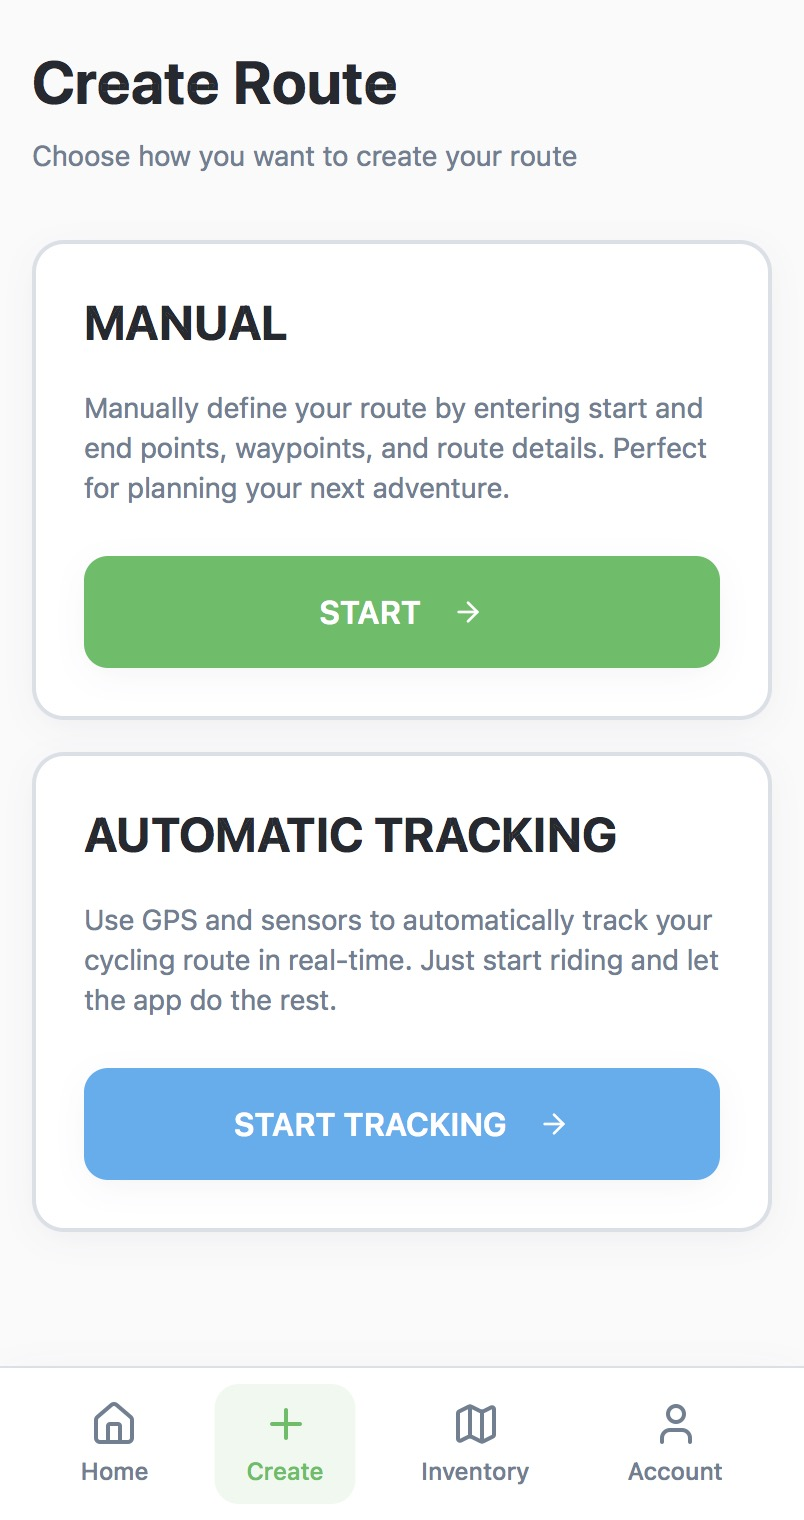
\includegraphics[width=0.34\textwidth]{Images/UserInterface/CreateRoute.JPG}
\hspace{1.3cm}
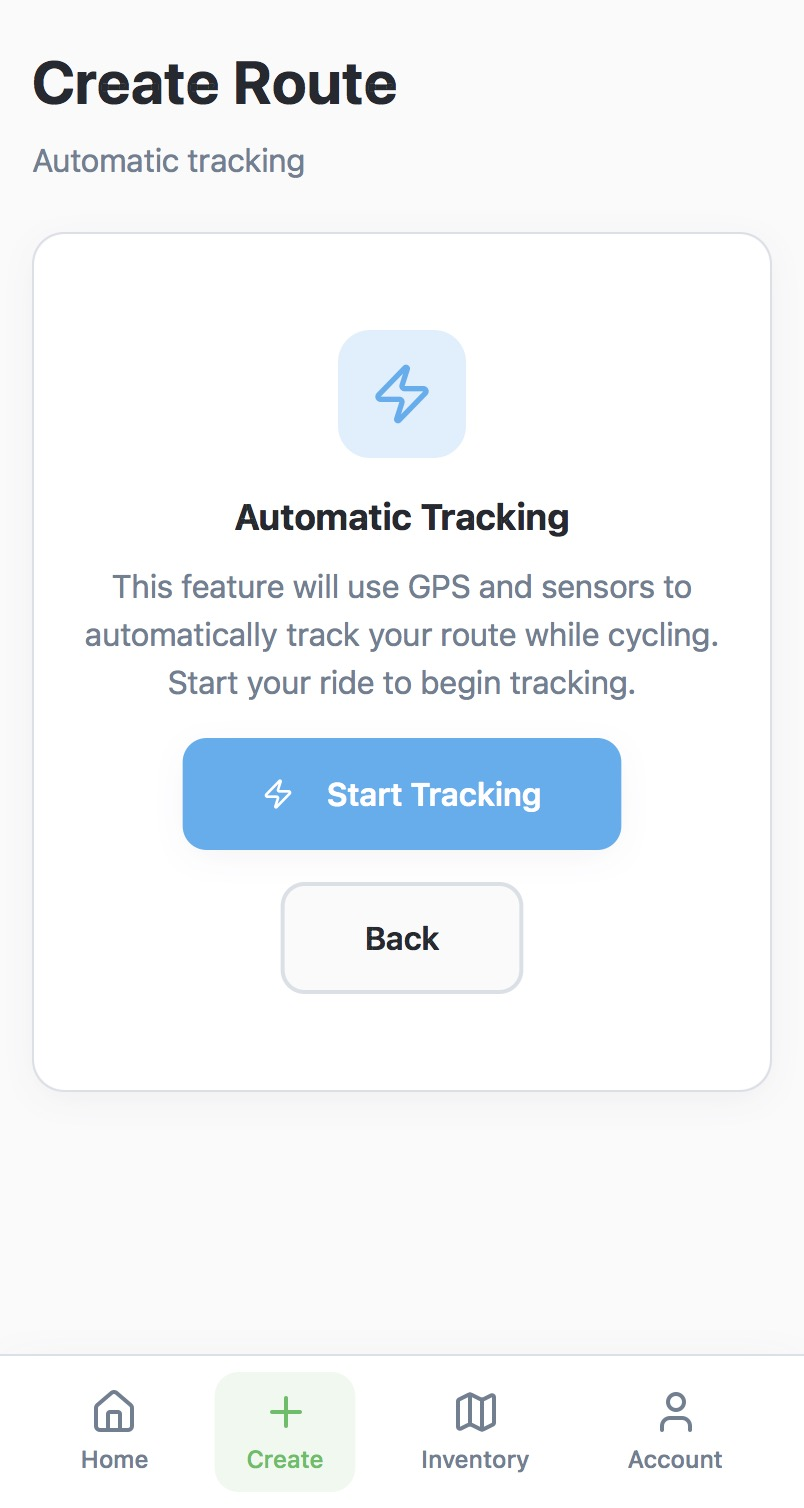
\includegraphics[width=0.34\textwidth]{Images/UserInterface/AM.JPG}
\caption{Screens of \textit{Create Route} and \textit{Create Route (Automatic Mode)}}
\label{fig:CreateRoute}
\end{figure}
\newpage
\begin{figure}[H]
\centering
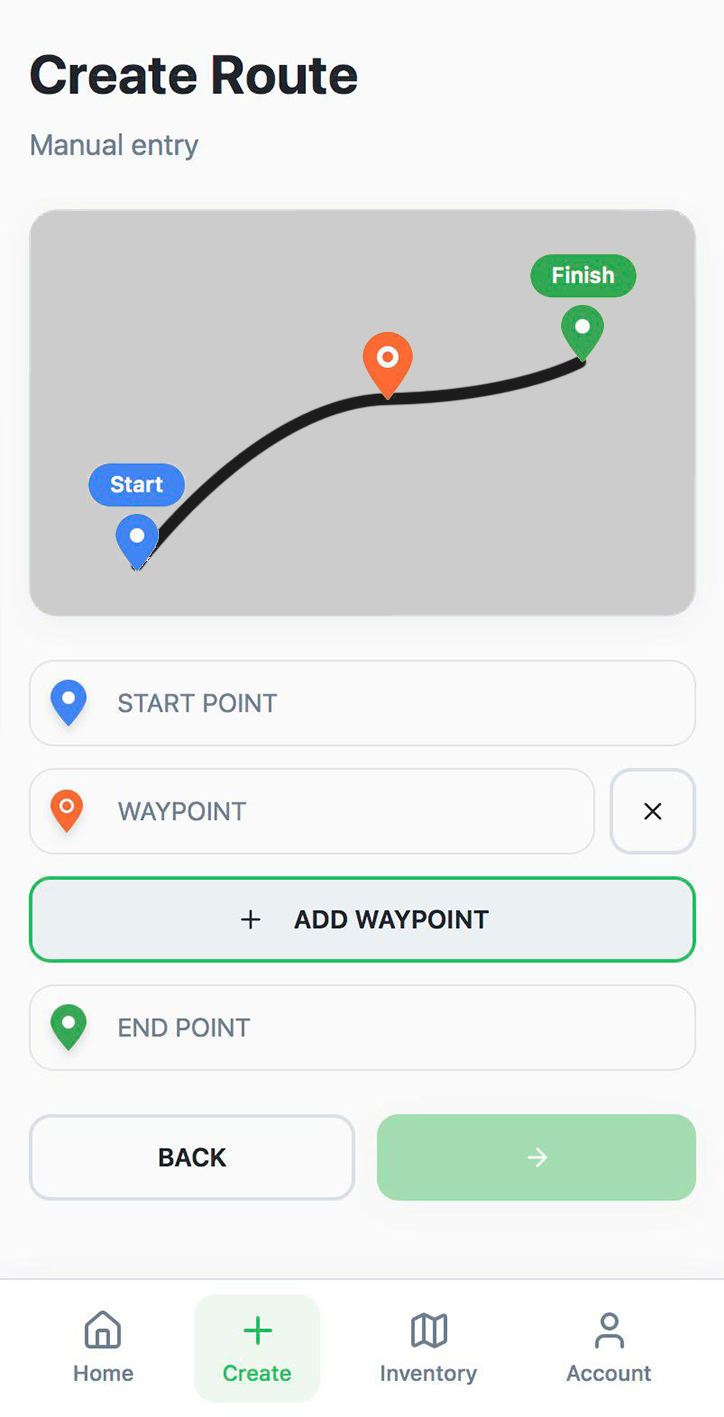
\includegraphics[width=0.34\textwidth]{Images/UserInterface/MM.JPG}
\hspace{1.3cm}
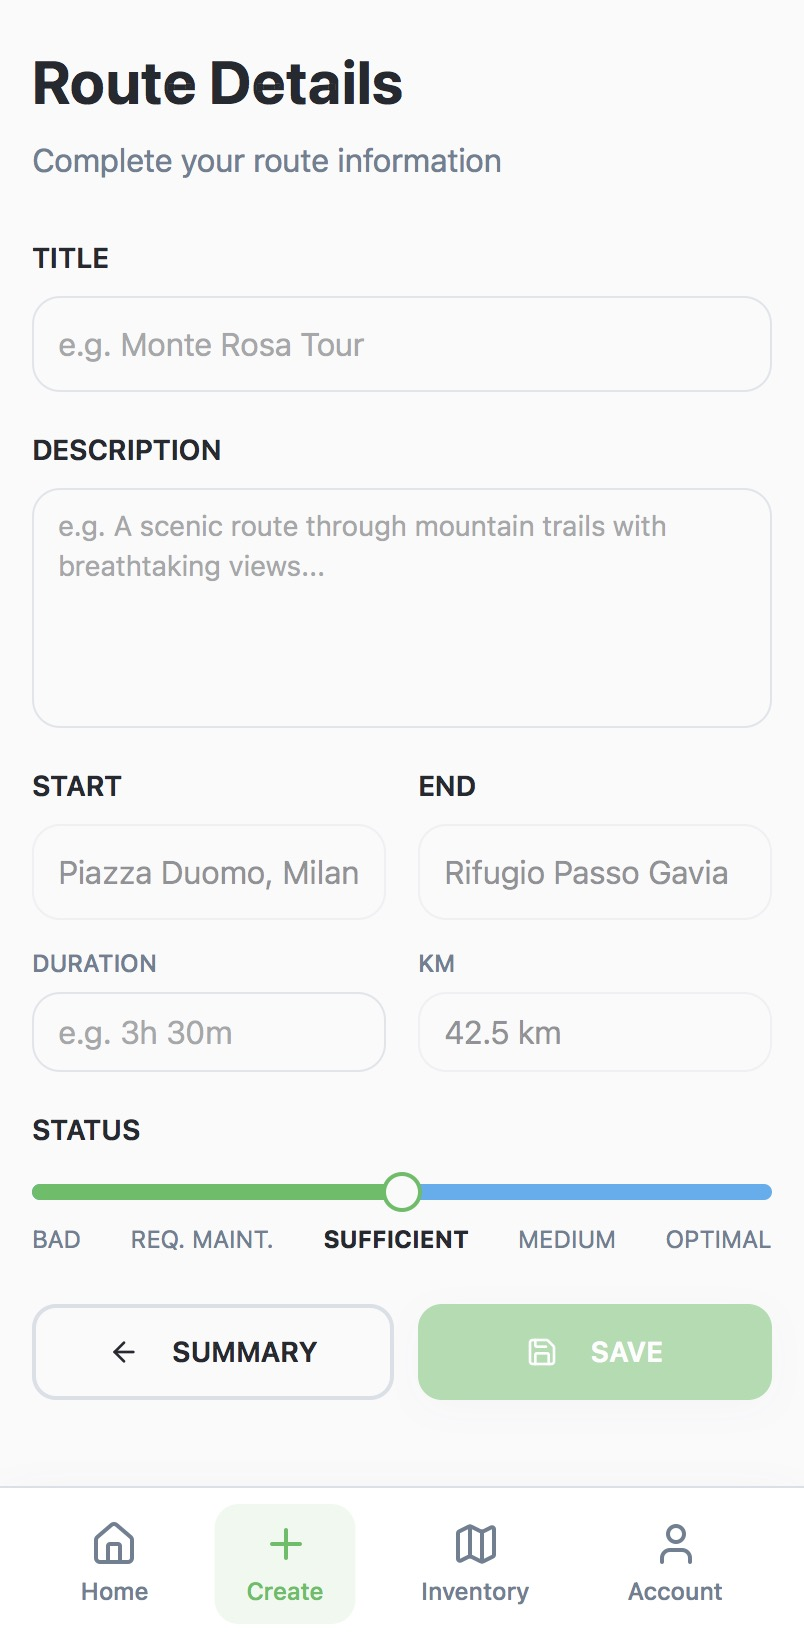
\includegraphics[width=0.34\textwidth]{Images/UserInterface/Details.JPG}
\caption{Screens of \textit{Create Route (Manual Mode)} and \textit{Route Details}}
\label{fig:CreateRouteManualDetails}
\end{figure}